\section{Results and Discussion}

\subsection{Show your synthetic image grids and denoising process images}

首先,展示模型根據測試資料集 test.json 與 new\_test.json 所生成的合成圖像網格。這些圖像旨在直觀地呈現模型在學習了數據分佈後,根據不同條件生成對應視覺內容的能力。

\begin{figure}[H]
    \centering
    \begin{subfigure}[b]{0.8\textwidth}
        \centering
        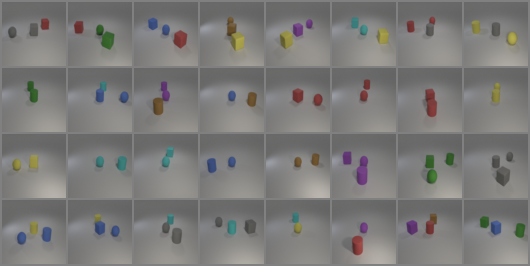
\includegraphics[width=\textwidth]{figures/new_test_result.png}
        \caption{new\_test.json 的生成結果}
        \label{fig:new_test_result}
    \end{subfigure}
    \vspace{1em} % 此指令用於在兩個子圖之間產生垂直間隔
    \begin{subfigure}[b]{0.8\textwidth}
        \centering
        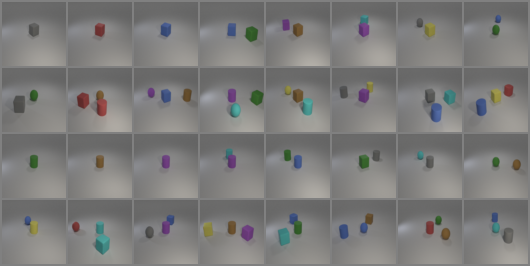
\includegraphics[width=\textwidth]{figures/test_result.png}
        \caption{test.json 的生成結果}
        \label{fig:test_result}
    \end{subfigure}
    \caption{模型為 test.json 與 new\_test.json 生成的合成圖像。}
    \label{fig:synthetic_images_grids}
\end{figure}

為了更深入地理解模型的學習過程,我進一步展示了在不同訓練階段(epochs)下,模型對於特定標籤組合 ``red sphere'', ``cyan cylinder'', ``cyan cube'' 的去噪過程。圖 \ref{fig:denoising_process} 由上至下依序呈現了模型在訓練了 100、500、2500 及 2700 個 epoch 後的去噪結果。從這些圖像中,我可以觀察到隨著訓練的進行,模型一開始是什麼都沒有學會,然後先生成了與方塊還有圓柱相似的物體,而且擺在圖片的後面,然後才學會放到圖片前,強調出稜角與圓角。

\begin{figure}[H]
    \centering
    \begin{subfigure}[b]{0.8\textwidth}
        \centering
        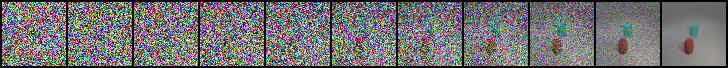
\includegraphics[width=\textwidth]{figures/ep100_25.png}
        \label{fig:ep100_25}
    \end{subfigure}
    \vspace{1em}
    \begin{subfigure}[b]{0.8\textwidth}
        \centering
        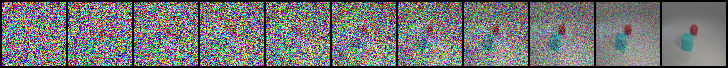
\includegraphics[width=\textwidth]{figures/ep500_25.png}
        \label{fig:ep500_25}
    \end{subfigure}
    \vspace{1em}
    \begin{subfigure}[b]{0.8\textwidth}
        \centering
        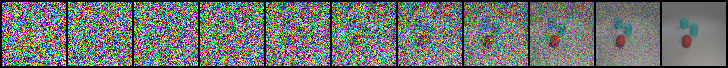
\includegraphics[width=\textwidth]{figures/ep2500_25.png}
        \label{fig:ep2500_25}
    \end{subfigure}
    \vspace{1em}
    \begin{subfigure}[b]{0.8\textwidth}
        \centering
        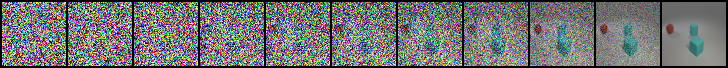
\includegraphics[width=\textwidth]{figures/ep2700_25.png}
        \label{fig:ep2700_25}
    \end{subfigure}
    \caption{不同訓練階段的去噪過程比較,標籤為 ["red sphere", "cyan cylinder", "cyan cube"]。從上到下分別為 epoch 100、500、2500 和 2700 的去噪過程。}
    \label{fig:denoising_process}
\end{figure}

\subsection{Evaluate your model with the classification accuracies}

除了視覺上的評估,我也使用了分類準確率來量化模型的性能。圖 \ref{fig:accuracy_plot} 展示了模型在測試集上的分類準確率隨訓練過程的變化,在接近 30 小時的訓練之後,我在 epoch 2700 時,得到了 98 \% 的準確率。

\begin{figure}[H]
    \centering
    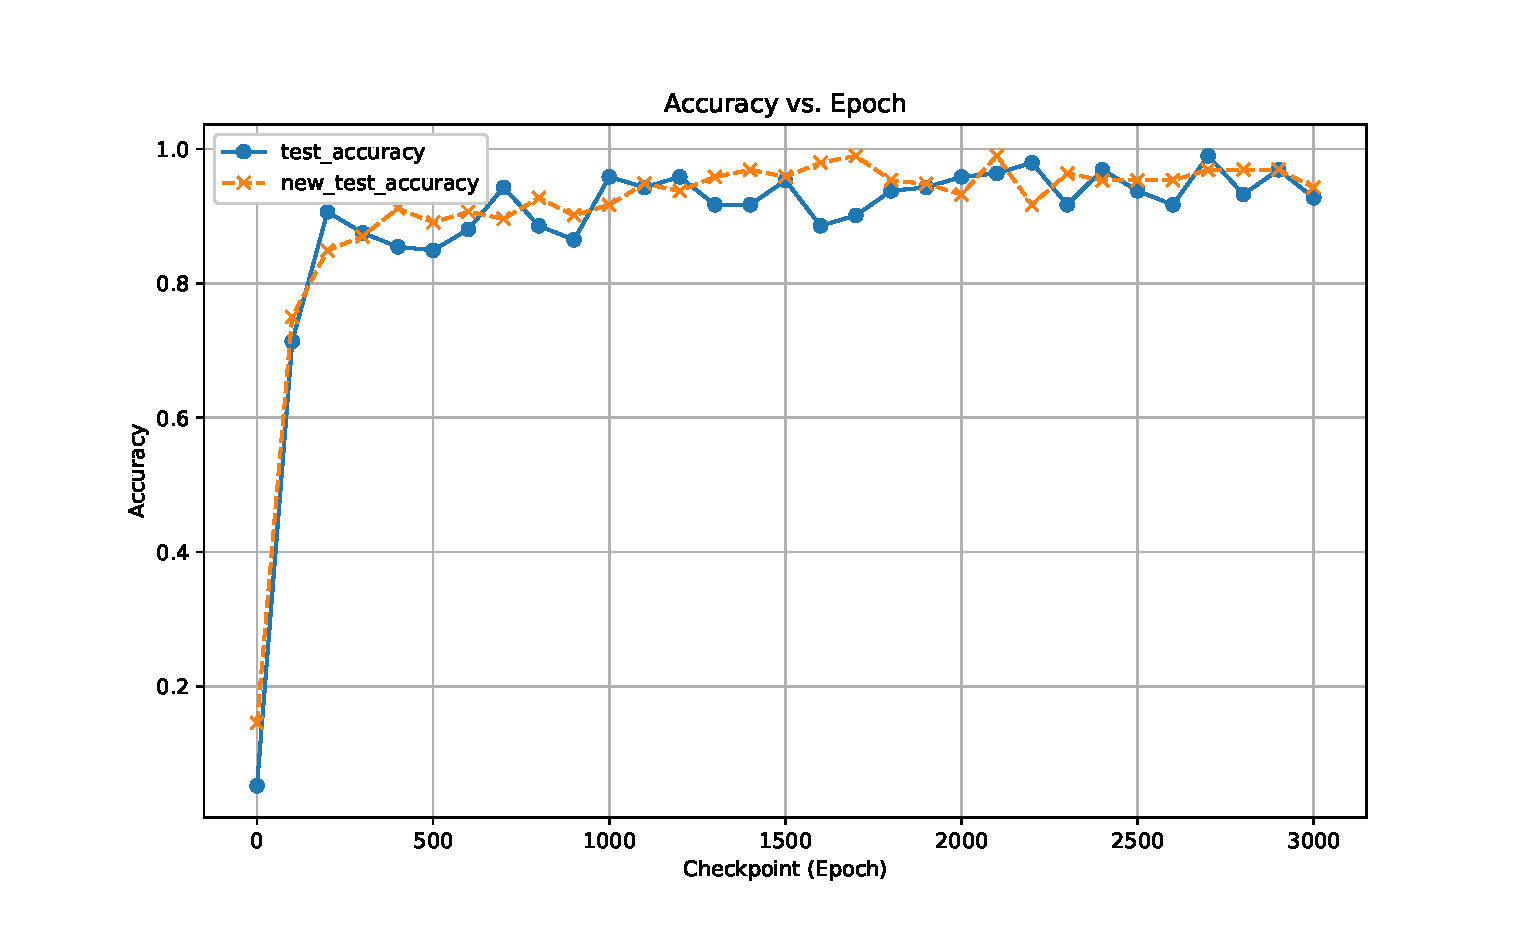
\includegraphics[width=0.8\textwidth]{figures/accuracy_plot.eps}
    \caption{模型在測試集上的分類準確率}
    \label{fig:accuracy_plot}
\end{figure}

\begin{figure}[H]
    \centering
    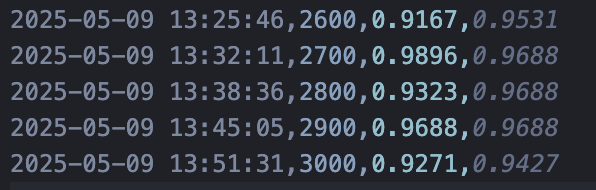
\includegraphics[width=0.8\textwidth]{figures/accuracy.png}
    \caption{模型在測試集上的分類準確率}
    \label{fig:accuracy}
\end{figure}


\subsection{Extra implementations and experiments: Training Details}

在一開始訓練的時候,當固定 epoch 的時候,會發現 batch size 越小的訓練 loss 越低,這讓我非常的困惑,那為什麼所有的論文都說 batch size 越大越好呢? 所以我猜測雖然 batch 小的收斂快,但是可能很容易卡在比較高的 local minimum,沒辦法更進一步,又或是因為 batch 比較小,所以會有很多次 update model 的機會,導致模型在訓練過程中,會有比較多的機會,可以更新模型,這樣可以讓模型學習到更多的資訊?

所以我固定了更新模型的次數,想要比較 batch\ size 16 vs 160 的差異,但是我發現我的電腦沒辦法訓練 batch 160,所以這裡我實作了 amp。圖~\ref{fig:different_bz} 初步展示了在不同 batch\ size 設定下訓練過程的比較,這有助於我理解 batch\ size 對模型學習效率和最終性能的潛在影響。

\begin{figure}[H]
    \centering
    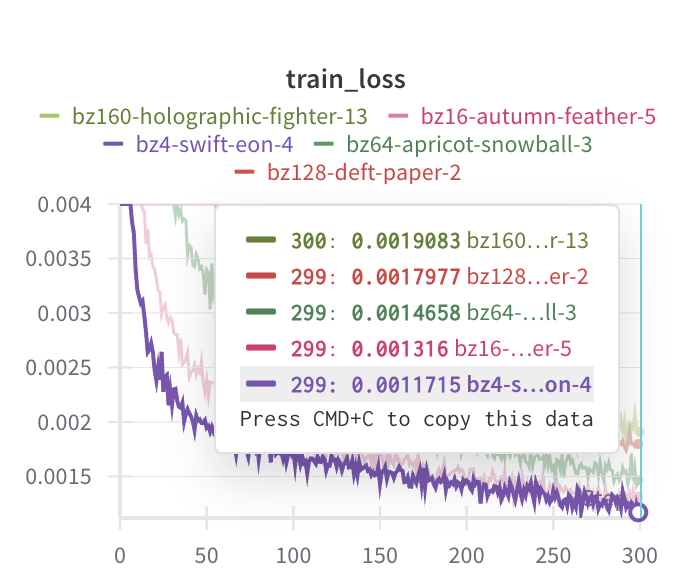
\includegraphics[width=0.8\textwidth]{figures/different_bz.png}
    \caption{不同 batch size 的訓練過程比較}
    \label{fig:different_bz}
\end{figure}

讓模型可以在 4090 的 24 G 記憶體上,訓練到 160 個 batch\_size,最終的結果也沒有辜負我的期望,可以在 41 秒跑完一個 epoch,這裡我訓練了 3000 個 epoch,可以達到 0.98 的準確率,會設計 3000 個 epoch 的原因是,batch 16 的 會比 batch 160 多更新模型 10倍的次數,這很明顯會對於 big batch 不利,所以我選擇讓更新的數量一樣,可以比較公平的比較。圖 \ref{fig:bz16vs160} 更細緻地比較了 batch size 為 16(子圖 \ref{fig:bz16_1})與 batch size 為 160(子圖 \ref{fig:bz16_2})時的訓練過程。透過這組比較,我可以更清晰地觀察在固定模型更新次數的前提下,不同 batch size 對訓練動態(如損失函數的下降速度、穩定性等)以及最終模型性能的具體差異。

\begin{figure}[H]
    \centering
    \begin{subfigure}[b]{0.48\textwidth}
        \centering
        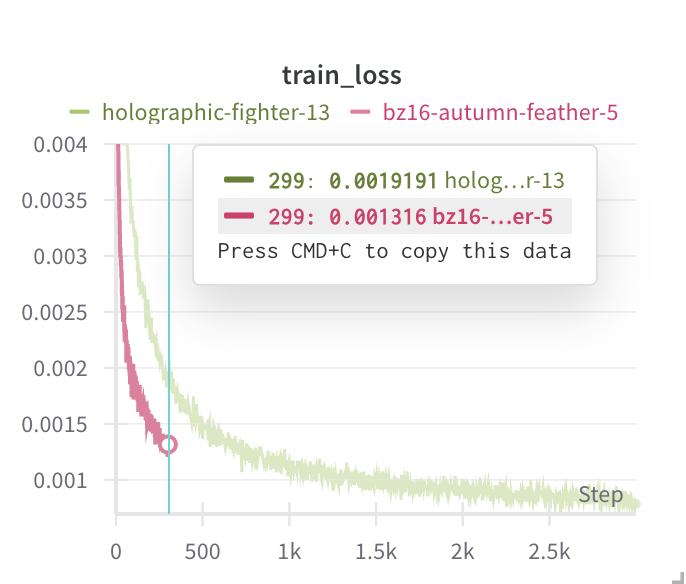
\includegraphics[width=\textwidth]{figures/bz16vs160_1.png}
        \caption{batch size 16 的訓練過程}
        \label{fig:bz16_1}
    \end{subfigure}
    \vspace{1em}
    \begin{subfigure}[b]{0.48\textwidth}
        \centering
        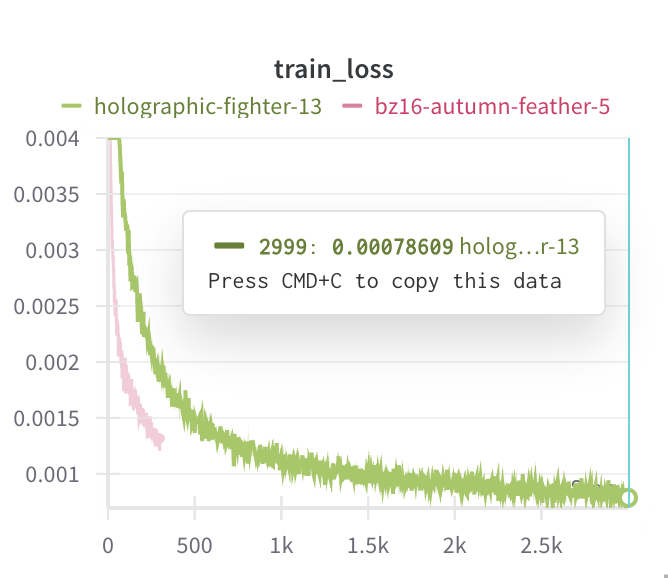
\includegraphics[width=\textwidth]{figures/bz16vs160_2.png}
        \caption{batch size 160 的訓練過程}
        \label{fig:bz16_2}
    \end{subfigure}
    \caption{不同 batch size 的訓練過程比較}
    \label{fig:bz16vs160}
\end{figure}




